\documentclass[conference]{IEEEtran}

\usepackage{cite}
\usepackage{graphicx}
\usepackage{tabularx, booktabs}
\usepackage{subfig}
\usepackage{algorithm}
\usepackage{algorithmic}
\hyphenation{op-tical net-works semi-conduc-tor}

\newcommand{\Comment}[1]{\textbf{#1}}
\setlength{\textfloatsep}{4pt plus 2pt minus 2pt}
\setlength{\floatsep}{4pt plus 2pt minus 2pt}
\setlength{\dbltextfloatsep}{4pt plus 2pt minus 2pt}
\setlength{\dblfloatsep}{4pt plus 2pt minus 2pt}
\begin{document}

\title{Performance Analysis of CNN Frameworks\\
 for GPUs}

\author{%
  \IEEEauthorblockN{Heehoon Kim$^{*\ddagger}$ $\quad$ Hyoungwook Nam$^{\dagger\ddagger}$ $\quad$ Wookeun Jung$^*$ $\quad$ Jaejin Lee$^*$}\\
  \IEEEauthorblockA{%
    $^*$Department of Computer Science and Engineering,\\
    $^\dagger$College of Liberal Studies,\\
    Seoul National University, Korea\\
    {\texttt \{heehoon, hyoungwook, wookeun\}@aces.snu.ac.kr, jaejin@snu.ac.kr}\\
    http://aces.snu.ac.kr
  }\\
  $^{\ddagger}$These two authors contributed equally to this work as the first authors.
}

\maketitle

\begin{abstract}
Thanks to modern deep learning frameworks that exploit GPUs, convolutional neural networks (CNNs) have been greatly successful in visual recognition tasks. In this paper, we analyze the GPU performance characteristics of five popular deep learning frameworks: Caffe, CNTK, TensorFlow, Theano, and Torch in the perspective of a representative CNN model, AlexNet. We identify the overhead of each framework and suggest possible optimization methods to increase the efficiency of CNN models built by the framework. We also show the GPU performance characteristics of four convolution algorithms each of which uses one of GEMM, direct convolution, FFT, and Winograd method. Based on the characterization, we suggest criteria to choose convolution kernels for GPUs and methods to build efficient CNN models on GPUs. Since scaling DNNs in a multi-GPU context becomes important, we also analyze the scalability of the deep learning frameworks in the multi-GPU context and their overheads. Based on the multi-GPU characterization, we suggest possible optimization methods for CNNs in the multi-GPU context.
\end{abstract}

\IEEEpeerreviewmaketitle

\renewcommand{\baselinestretch}{.95} 
\section{Introduction}

Deep neural networks (DNNs) have been very successful on various machine learning tasks, such as visual recognition\cite{krizhevsky2012imagenet,vgg,RCNN}, speech recognition\cite{speech}, and machine translation\cite{machinetranslation}.
Among others, the convolutional neural network (CNN) proposed by LeCun \textit{et al.}\cite{726791}, is one of the earliest successful DNN models that were used to classify images.
CNN models equipped with deep learning techniques (\textit{e.g.}, ReLU activation, dropout layers, data augumentation, etc.) outperform previous machine learining techniques in various visual recognition challenges, such as ILSVRC\cite{DBLP:journals/corr/RussakovskyDSKSMHKKBBF14} and PASCAL\cite{pascal}.
The classification accuracy of CNN models have been improving over time.
In addition, recent state-of-the-art techniques for visual recognition use an ensemble of different CNN models\cite{ILSVRC15}.
CNN models are also being applied to other machine learning tasks than image recognition.
They can also be applied to action recognition\cite{actionrecognition}, speech recognition\cite{speech}, natural language processing\cite{DBLP:journals/corr/KalchbrennerGB14}, and playing Go\cite{alphago}.

The biggest advantage of using DNN is its scalability.
A larger and deeper DNN with more parameters usually results in a better accuracy.
However, a larger DNN require more processing power, and training it using a typical computer is impractical.
Fortunately, computations in a neural network can easily be represented as tensor or matrix operations that can be efficiently parallelized.
Thus, GPUs' massively parallel processing power make DNNs to be trained efficiently even in a single desktop computer.
Since deep learning frameworks have been developed for the efficient and easy implementation of DNN models, most of popular deep learning frameworks support GPU acceleration by default\cite{DBLP:journals/corr/Al-RfouAAa16,jia2014caffe,tensorflow2015-whitepaper,torch,cntk}.
As a result, companies and researchers have been trying to implement efficient GPU kernels to improve the performance of deep learning frameworks.

The most popular deep learning library for such frameworks is cuDNN\cite{cudnn}.
It has been developed by NVIDIA, and most of the popular deep learning frameworks use it as the backend for GPUs.
For example, computing convolution with cuDNN results in up to 4X performance improvement compared with the default GPU kernels of the frameworks\cite{convnet-benchmarks}.
Another approach to speed up CNNs is reducing the time complexity of convolution algorithms.
Fast Fourier Transform (FFT) algorithms\cite{fftconv, fbfft} and Winograd's minimal filtering algorithm\cite{winograd} successfully reduce the time complexity of the convolution computation.
However, while the efficiency of deep learning on a single GPU has been improved a lot, deep learning on multiple GPUs still shows poor scalability\cite{DBLP:journals/corr/YadanATR13}.

In this paper, we analyze the performance characteristics of CNNs on different deep learning frameworks and libraries.
For clarity, a \textit{framework} refers to a full collection of libraries to build DNN models and a \textit{library} refers to a GPU kernel library such as cuDNN used for the framework.
We choose five most popular deep learning frameworks, Caffe\cite{jia2014caffe}, CNTK\cite{cntk}, TensorFlow\cite{tensorflow2015-whitepaper}, Theano\cite{DBLP:journals/corr/Al-RfouAAa16}, and Torch\cite{torch}.
The criterion for popularity is the number of github\cite{github} stars.
We also choose a CNN model, AlexNet\cite{krizhevsky2012imagenet}, to obtain the performance characteristics from the frameworks and libraries.
Identically structured AlexNet models are built and trained using these frameworks.
All the five frameworks use cuDNN as the GPU backend.
Cuda-convnet\cite{cuda-convnet} developed by Alex Krizhevsky is another GPU library used in this paper.
In addition, we compare three different convolution algorithms of cuDNN with the direct convolution algorithm of cuda-convnet.

The contributions of this work can be divided into three parts.
First, we analyze differences in the performance characteristics of the frameworks.
We identify performance limiting factors of each framework and describe pros and cons of using each deep learning framework for propspective users.
The performance limiting factors would also be helpful to optimizing the frameworks.
Second, we obtain the performance characteristics of different convolution algorithms.
Based on the result of analyzing the charateristics, we provide possible optimization techniques to implement efficient CNN models using the libraries.
Finally, we obtain the performance characteristics of the frameworks in multi-GPU contexts. We also provide possible techniques to improve the scalability of the frameworks when using multiple GPUs.

\section{Background and Related work}

\subsection{Previous work}
It has been only a few years since deep learning frameworks were introduced to public.
Few attempts recently tried to benchmark and compare the performance of the frameworks.
A benchmark of CNN frameworks is publicly available on Github\cite{convnet-benchmarks}.
It shows forward and backward propagation time of CNN model for each framework.
But the latest result was tested with cuDNN version R4, while the most recent version is R5.1.
Detailed benchmarks of deep learning frameworks were recently published\cite{DBLP:journals/corr/BahrampourRSS15, DBLP:journals/corr/ShiWXC16}.
They show execution times of various DNN models run on the frameworks.
However, the benchmarks show only the results, without identifying the reasons for the differences.
They also use cuDNN version of R4, which do not support most recent Winograd convolution.


\subsection{Machine learning frameworks}

Theano is a python framework for evaluating mathematical expressions\cite{DBLP:journals/corr/Al-RfouAAa16}.
It is one of the earliest framework used to build DNN models.
Multiple machine learning frameworks are built on top of Theano.
Pylearn2, Keras and Lasagne are popular frameworks for DNN using Theano as their backend.
Multiple GPU support of Theano is still on experimental stage.
Torch is a scientific computing framework based on LuaJIT\cite{torch}.
Torch is also one of the earliest frameworks used to implement CNN models.
Nvidia's self-driving car project and Deepmind's Deep Q Learning model were built on Torch\cite{nvdave, mnih2015humanlevel}.
Torch natively supports multi-gpu context via its cutorch module.
Caffe is deep learning framework developed by Berkeley Vision and Learning Center\cite{jia2014caffe}.
Caffe use prototxt file to describe DNN models.
Pre-trained network models can be imported with prototxt files.
Visual recognition challenge winners are usually implemented by Caffe\cite{ILSVRC15, RCNN, vgg}.
The flexibility of Caffe is limited.
Introducing a new feature to a layer requires re-building of the entire source code.
The multi-gpu support of Caffe is limited to batch data parallelism.
Tensorflow is machine learning framework developed by Google\cite{tensorflow2015-whitepaper}.
It was first introduced to public in 2015, and is now the most popular machine learning framework on GitHub.
Tensorflow supports both Python and C++ interface.
Computational Network Toolkit(CNTK) is deep learning framework developed by Microsoft\cite{cntk}.
CNTK supports both Windows and Linux environment, while the others do not support Windows.
CNTK uses its own BrainScript to describe DNN models.
It also supports C++ and C\# wrappers to evaluate models.

\begin{figure}
  \centering
  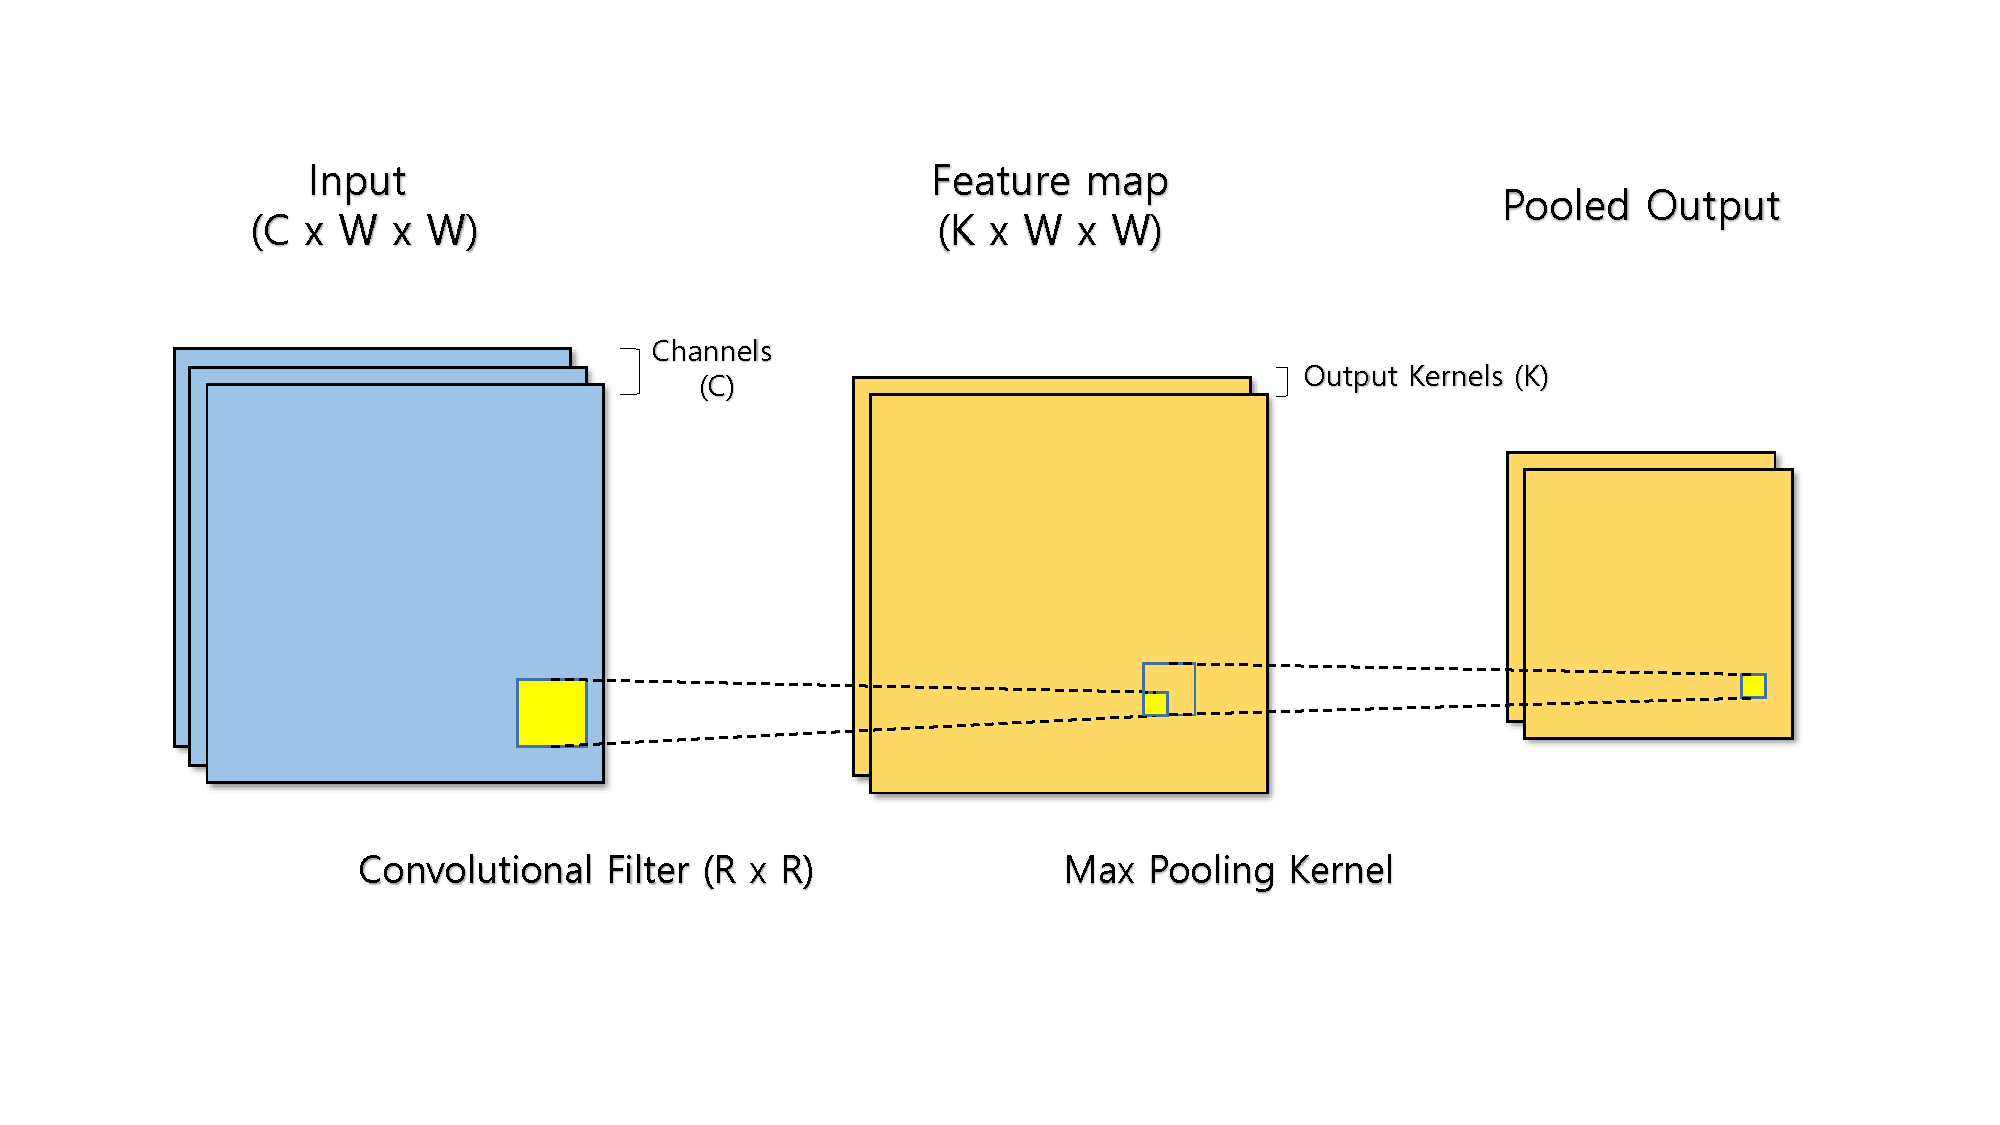
\includegraphics[width=\linewidth]{./figures/conv_2dlayer}
  \caption{An example of typical 2D convolution layer. }
  \label{fig_convlayer}
\end{figure}
\begin{figure}
  \centering
  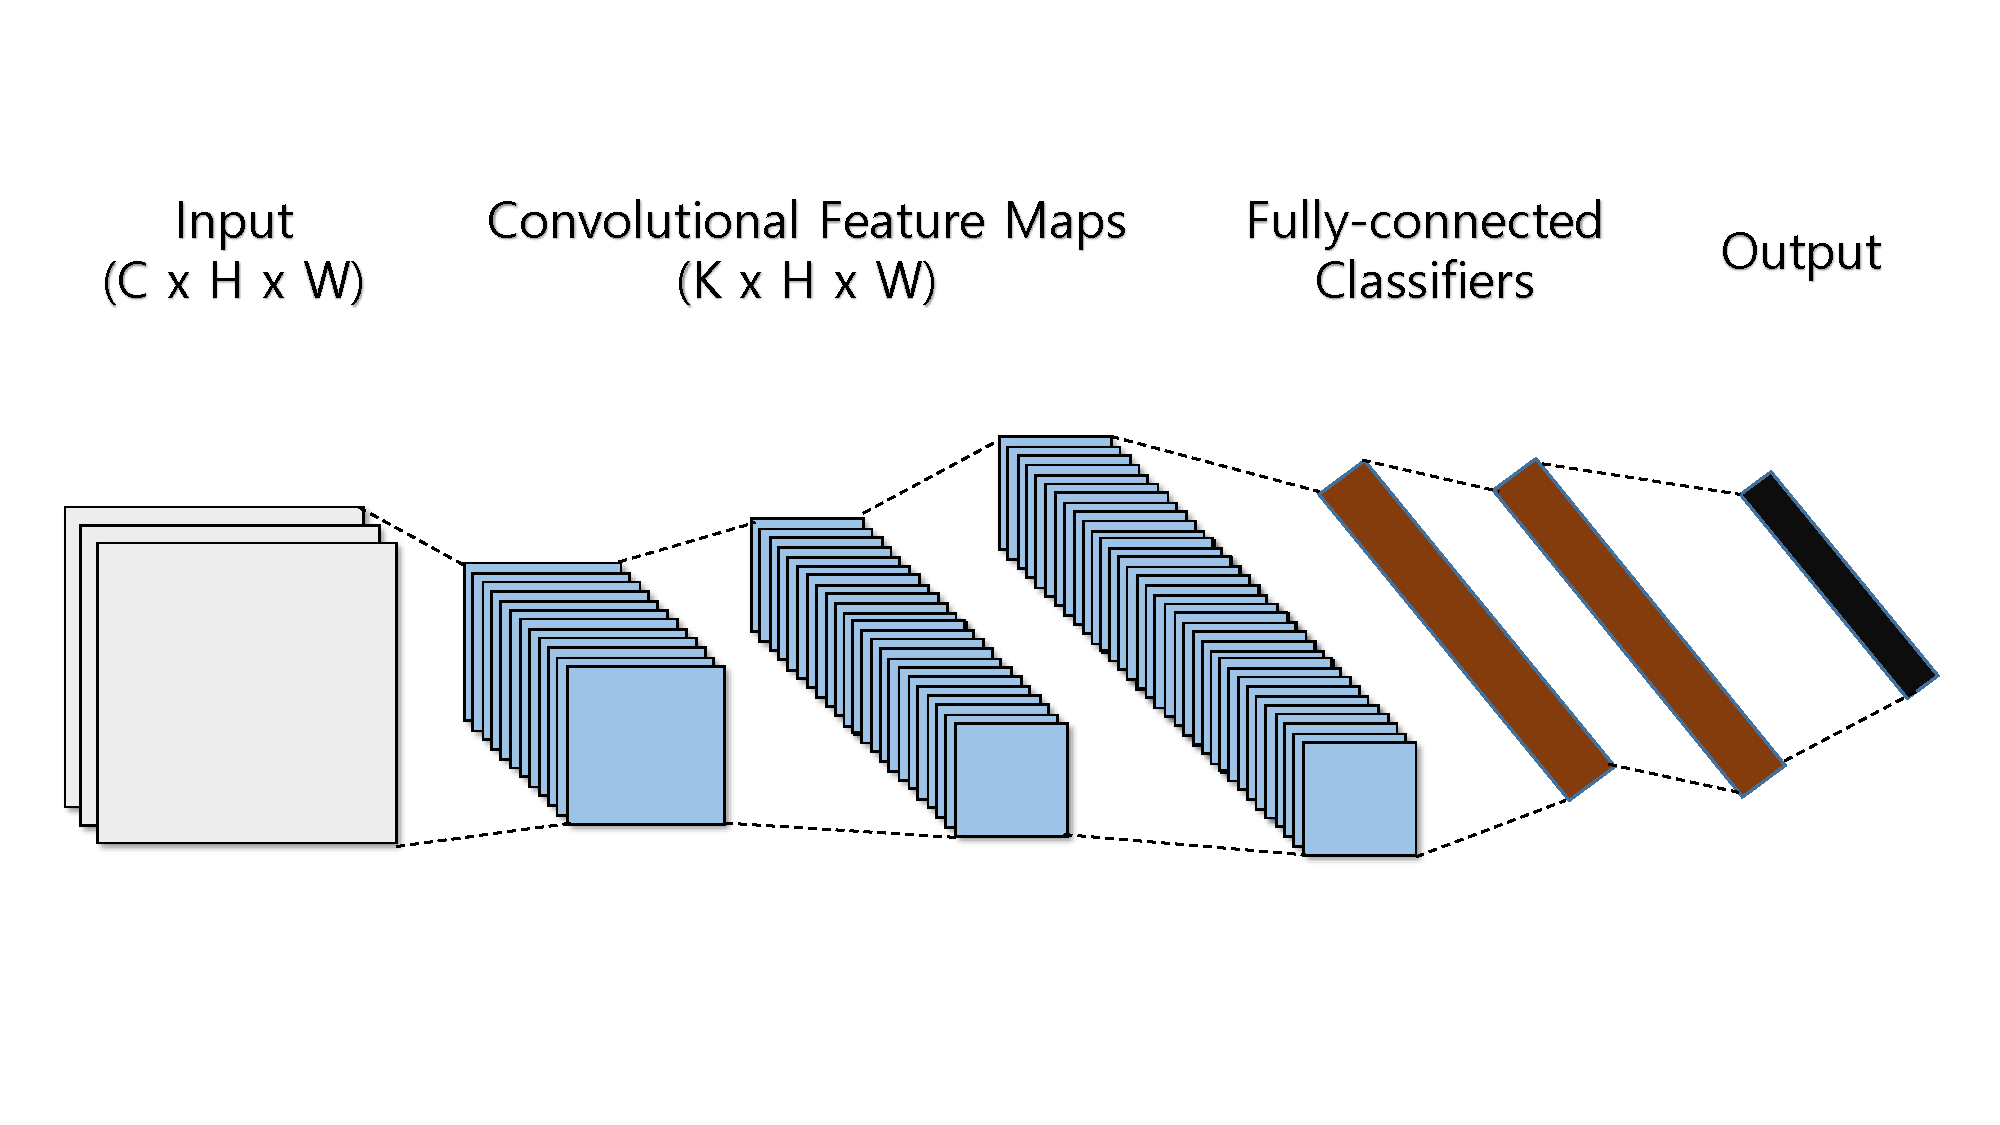
\includegraphics[width=\linewidth]{./figures/conv_model}
  \caption{A typical CNN network model }
  \label{fig_convmodel}
\end{figure}

\subsection{Convolutional Neural Network}
Convolutional Neural Network(CNN) is an Artificial Neural Network using convolutional filter to extract features from input.
Convolution is an operation between two functions which creates a new function defined as an integration of translated pointwise multiplication of two functions.
\begin{equation}
\left ( f * g \right )(t) = \int f(x)g(t-x)dx = \int f(t-x)g(x)dx
\label{def_convolution}
\end{equation}
Convolution of two finite sequences can be defined as follows.
\begin{equation}
\lbael{def_discrete}
\left ( f * g \right )[n] = \sum_{1}^{M} f[n + m]g[m]
\end{equation}
Convolution can be extended to multiple dimensions.
A 2D convolution between filter F[R][S] and data D[H][W] can be described with following equation.
\begin{equation}
\lbael{def_2d}
\left ( D * F \right )[h][w] = \sum_{1}^{R}\sum_{1}^{S} D[h + r][w + s] F[r][s]
\end{equation}

Convolutional neural network on 2D images uses 2D spatial convolution.
2D spatial convolution is 3-dimensional convolution with the third axis for input channels.
A batch input of 2D spatial convolution is typically formatted as a 4D tensor of <batch, channel, height, width>(NCHW).
Figure \ref{fig_convlayer} shows an example of 2D spatial convolutional layer.
K filters of filter size R * R convolves among input data of dimension W * W.
Each convolutional filter activation corresponds to a channel of output feature map.
A nonlinear activation function is applied to calculate an activation of a filter.
Most CNN use Rectified Linear Unit(ReLU) for nonlinear activation to avoid vanishing gradient problem\cite{rectified}.
A convolution by stride S and padding P creates a feature map of dimension (W - R + P + 1)/S with K channels.
Usually a pooling layer is applied to create an output feature map of reduced dimension.
Output feature map is usually formatted to a same NCHW 4D tensor, which can be used as input data for next convolution layer.
The computational complexity of computing such convolutional layer is O(K * CRR * NWW).

\subsection{Convolution algorithms}
Several methods are used to efficiently implement convolution on GPU.
Direct convolution is the most straightforward way but needs a lot of specialized kernels to optimize for various input dimensions and corner cases.
Cuda-convnet \cite{cuda-convnet} is the efficient direct convolution library written by Alex Krizhevsky, the author of AlexNet paper.
CuDNN however, treats convolution as matrix multiplication(GEMM) \cite{cudnn}.
The convolution layer of K kernels with dimension R*R and W*W input with C channels is converted to multiplication of K*CRR filter matrix and CRR*NWW data matrix.
The dimensions of matrices are very big, hence the multiplication can be parallelized using highly efficient BLAS libraries.
Converting convolution to matrix might require significant amount of memory bandwidth.
CuDNN computes the multiplication by tiles to hide memory latency while computing.
This method scales well on small batch sizes and can be used on all types of convolution layers.
The complexity of both methods are basically the same.

FFT convolution uses fast Fourier transform algorithm to reduce algorithm complexity \cite{fftconv}.
Typical convolution has algorithm complexity of O(K * CRR * WW), while FFT convolution shows complexity of O(K * CWW * log(W)) which does not depend on the size of the filter.
FFT convolution requires more memory space since filters must be padded to the dimension of inputs.
However, FFT convolution cannot be applied to convolution with stride more than 1.
Winograd convolution algorithm is based on GEMM convolution but reduces algorithm complexity using Winograd's minimal filtering algorithm.
Using Winograd’s minimal filtering algorithm, matrix multiplication of 4x3 tiled matrix requires 6 multiplications instead of 12.
Nesting the minimal filtering algorithm reduces 12*12 multiplications into 6*6 multiplications, reducing algorithm complexity by 4 \cite{winograd}.
However, different sized kernel needs its own minimal filtering algorithm, hence CuDNN 5.1 only supports Winograd convolution for filter size of 3x3 and 5x5.

\subsection{Multi-gpu parallelism}
Multi-gpu implementation of deep neural networks can be implemented by data parallelism or model parallelism \cite{NIPS2012_4687}.
On data parallelism, a batch of inputs is divided and distributed among devices.
After backpropagation, the entire gradients of network parameters must be passed to single device in order to compute stochastic gradient descent.
And then the updated parameters are distributed among devices.
Hence, the communication cost of data parallelism depends on number of parameters in the network.
AlexNet has 65M parameters, thus each iteration needs to transfer approximately 520MB of data per GPU.
On the other hand, model parallelism divides and distributes the network on each GPU.
Since parameter updates can be done on each GPU, only a small amount of activation data is communicated between GPU.
Carefully designed model parallelism of convolution layer outperforms the data parallelism \cite{DBLP:journals/corr/YadanATR13}.
However, multi-gpu support on Caffe is limited to data parallelism, therefore we only compare data parallelism efficiencies of the frameworks.
Tensorflow and Torch supports both data and model parallelism while Theano doesn’t support multi-gpu natively.


\section{Experiment setup}

\subsection{System setup}
We test the frameworks on the CentOS 7.2 server with 4 octa-core Xeon-E5 cpus and 4 GTX TITAN X(GM200) gpus.
We use Cuda 7.5 and CuDNN R5 which is the latest stable release of Cuda and CuDNN.
All deep learning frameworks are updated to latest stable release on June 2016.
The versions of the frameworks fully support CuDNN R5.
Only Torch supports the latest version of Cuda-convnet3.
The detailed system environments are represented on Table \ref{} and \ref{}.

CentOS 7.2.1511 / Linux 3.10.0-327 / Inte Xeon E5-2650@2.0GHz / 128GB DDR3@1600MHz / CuDNN 5005 / Cuda 7.5 / Torch 7 ccn2.torch, cudnn.torch R5 / Theano 0.8.2 / Caffe * / Tensorflow *
%TODO

\subsection{AlexNet model}
AlexNet \cite{} is one of the earliest successful deep neural networks on image recognition task using ImageNet dataset \cite{}.
AlexNet uses 5 convolution layers to extract features and 3 fully connected layers for classification.
Each layer has rectified linear unit(ReLU) layer for nonlinear activation.
AlexNet has been frequently used for benchmarking performance of machine learning libraries, because it utilizes most of the current DNN components such as convolution, max-pooling and dropout \cite{}.
The original AlexNet model includes Local response normalization(LRN) layer, but we exclude it for benchmarking task since LRN is very rarely used in current convolutional neural networks.
The detailed layer structure of AlexNet model on this study is presented in Table \ref{}.


\begin{table*}[]
\centering
\caption{Alexnet model used on benchmarking}
\label{alex_model}
\begin{tabular}{llllllll}
Name    & Kernel(R) & Input Channels(C) & Ouput Channels(K) & Stride(K) & Sample width(W) & Params & Flop \\
Input   &           & 3                 &                   &           & 227 x 227       &        &      \\
Conv1   & 11 x 11   & 3                 & 96                & 4         & 55 x 55         & 35K    & 55G  \\
Pool    & 3 x 3     &                   &                   & 2         &                 &        &      \\
Conv2   & 5 x 5     & 96                & 256               & 1         & 27 x 27         & 614K   & 227G \\
Pool    & 3 x 3     &                   &                   & 2         &                 &        &      \\
Conv3   & 3 x 3     & 256               & 384               & 1         & 13 x 13         & 885K   & 65G  \\
Conv4   & 3 x 3     & 384               & 384               & 1         & 13 x 13         & 1.3M   & 98G  \\
Conv5   & 3 x 3     & 384               & 256               & 1         & 13 x 13         & 885K   & 65G  \\
Pool    & 3 x 3     &                   &                   & 2         &                 &        &      \\
FC6     &           & 256 x 6 x 6       & 4096              &           &                 & 37M    & 74M  \\
FC7     &           & 4096              & 4096              &           &                 & 16M    & 32M  \\
FC8     &           & 4096              & 1000              &           &                 & 4M     & 8M   \\
Softmax &           & 1000              & 1000              &           &                 &        &     
\end{tabular}
\end{table*}

\begin{figure*}[htbp]
  \centering
  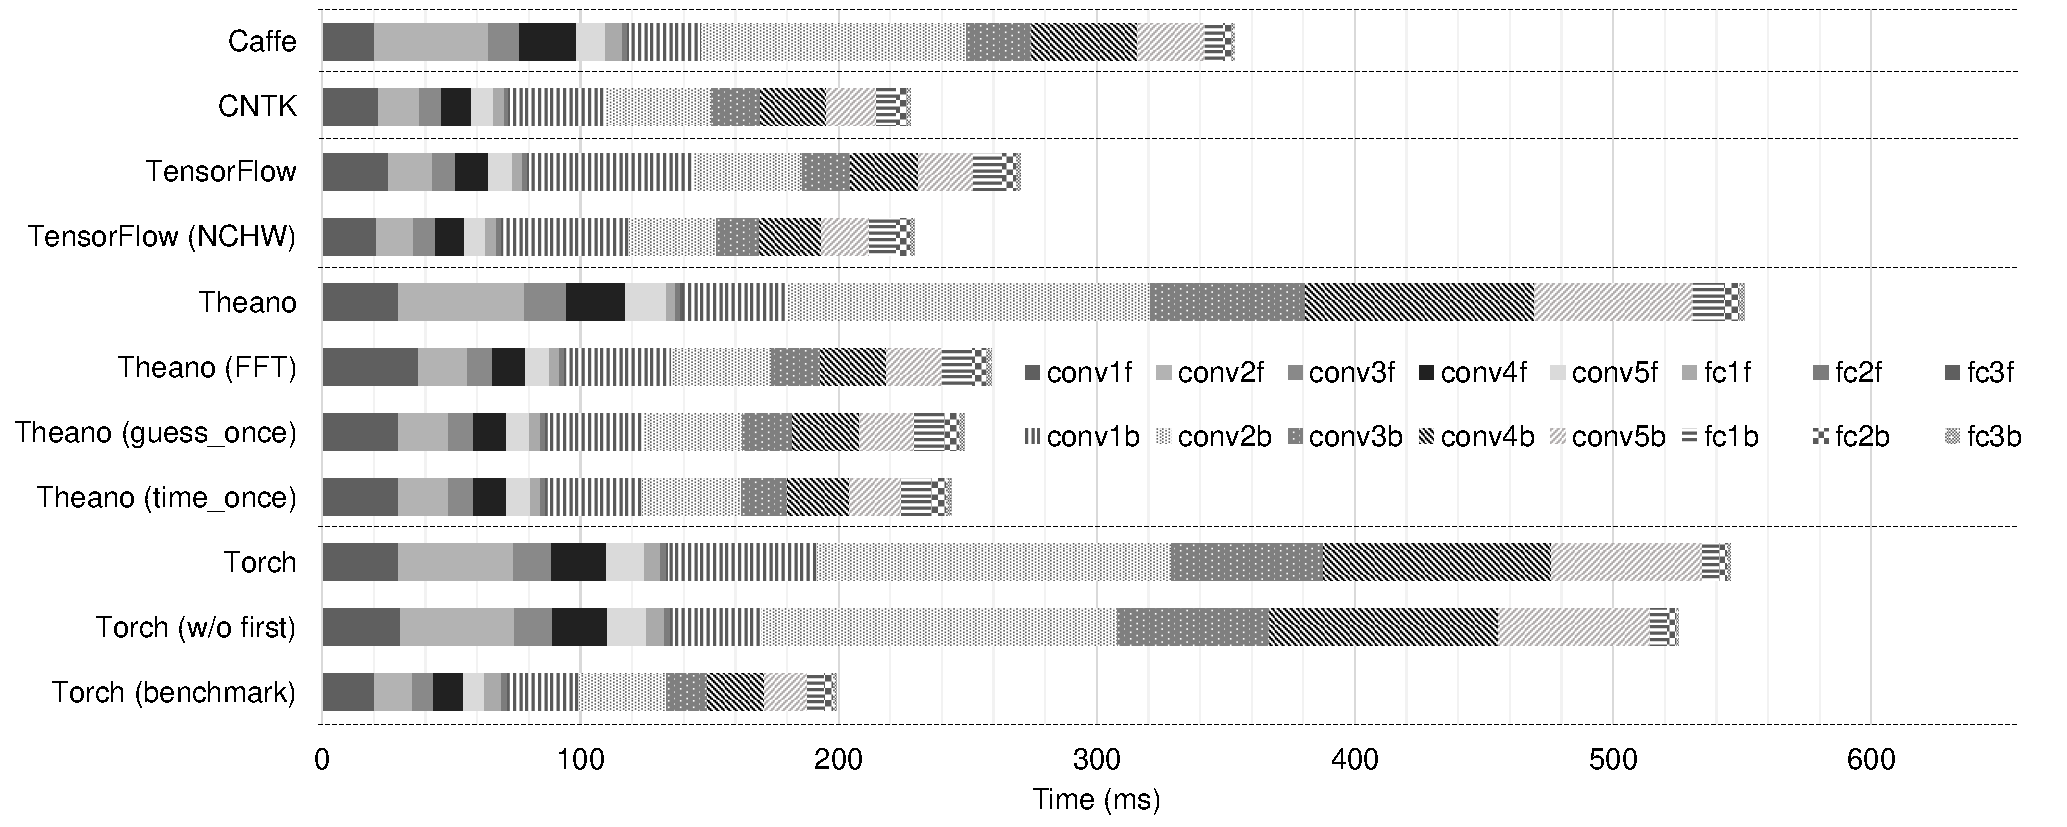
\includegraphics[width=\linewidth]{./figures/time_frameworks}
  \caption{%
The execution time of training AlexNet with a batch of imput images for differnt deep learning frameworks. 
\label{fig_time_frameworks}
  }
\end{figure*}

%A = Caffe, B = TensorFlow, C = TensorFlow (NCHW tensor), D = Theano, E = Theano (FFT), F = Theano (guess\_once), G = Theano (time\_once), H = Torch, I = Torch (no backward propagation in the first layer), J = Torch (FFT), K = Torch (benchmarking) 

\section{Charactrization on a Single GPU}
\label{sec:singlGPU}
In this section, we characterize the five deep learning frameworks on a single GPU. The measurement of the layer-wise execution time of the AlexNet model for each framework is shown in Figure~\ref{fig_time_frameworks}. The batch size of 256 was used in the experiment. The string in parentheses after the framework name stands for the framework configuration when the AlexNet model is built. No parentheses means the default options. A bar shows the breakdown of the total execution time into that of each layer. A layer name suffixed with \textsf{f} stands for the forward computation stage, and \textsf{b} for the backward computation stage.

\subsection{Options for Convolution Algorithms}
{\bf Caffe}. Caffe does not have any explicit option to choose convolution algorithms. Instead, it exploits cuDNN's heuristics that try to determine the best suited algorithm under the given specification of the model. Surprisingly, Caffe does not have an appropriate memory management technique yet. As result, algorithms that require a smaller memory space, such as GEMM and Winograd, can be inappropriately selected resulting in low performance even if Caffe exploits cuDNN's heuristics. 

{\bf TensorFlow}. TensorFlow also does not provide any option to choose convolution algorithms. Unlike Caffe, however, it executes all available algorithms in the first run by itself. Then, the fastest algorithm for each layer is executed in subsequent runs. The FFT algorithm is chosen for all the convolution layers except \textsf{conv1}, where FFT cannot be used because of the stride size (4). Since the set of algorithms that can be chosen is fixed and hardwired, recently added options of cuDNN R5.1 are not included in the set.

{\bf Theano}. On the other hand, Theano provides full accesses to the choices of convolution algorithms. Users can specify a specific convolution algorithm globally or in a layer-by-layer manner. There are two types of GEMM implementations in cuDNN: explicit and implicit. Theano selects the explicit GEMM by default. When a convolution algorithm is given as a global option, and the algorithm does not match the condition for a layer, the implicit GEMM is chosen as a fallback for the layer. However, the implicit GEMM is usually slower than the explicit GEMM. Thus, it is better to give layer-wise option to make Theano not to choose the implicit GEMM. \textsf{Theano (FFT)} in Figure~\ref{fig_time_frameworks} stands for the AlexNet model built by Theano with a global option for the FFT algorithm. However, \textsf{conv1} cannot use the FFT algorithm because of its stride size. Instead, the implicit GEMM is chosen for \textsf{conv1}. This is the reason why \textsf{conv1} of \textsf{Theano (FFT)} in Figure~\ref{fig_time_frameworks} is slower than those of \textsf{Theano (guess\_once)}, \textsf{Theano (time\_once)}, and even \textsf{Theano}. 

Unlike Caffe, Theano properly exploits cuDNN's heuristics when the \textsf{guess\_once} option is given. The \textsf{guess\_once} option makes Theano behave like Caffe where cuDNN's heuristics determine the best suited algorithm. The \textsf{time\_once} option in Theano exploits cuDNN's another functionality that executes all available convolution algorithms and choose the fastest one. Unlike TensorFlow, the set of algorithms in Theano is not hardwired. When the \textsf{time\_once} option is on, Theano uses GEMM in the first layer. It uses FFT or Winograd for the rest of the convolution layers. When the \textsf{guess\_once} option is on, the selection of an algorithm for each layer is slightly different from \textsf{time\_once}, but the execution time is almost the same as that of \textsf{time\_once}. This implies that cuDNN's heuristics are quite reliable.

\begin{table}[htbp]
\centering
\caption{Other GPU Kernels}
\label{table_misc_kernel}
\begin{scriptsize}
\begin{tabular}{|l|l|l|l|l|l|}
\hline\hline
           & Caffe    & CNTK    & TensorFlow & Theano  & Torch \\ \hline\hline
Bias       & cuDNN    & CNTK    & TensorFlow & Theano  & cuDNN \\ \cline{2-6} 
addition   & 2.64 ms  & 4.74 ms & 2.84 ms    & 7.88 ms & 2.63 ms  \\ \hline\hline
ReLU       & cuDNN    & CNTK    & Eigen      & Theano  & cuDNN \\ \cline{2-6}
activation & 2.56 ms  & 2.26 ms & 2.43 ms    & 4.59 ms & 2.56 ms  \\ \hline
\end{tabular}
\end{scriptsize}
\end{table}

Although Theano executes the fastest algorithm for convolution computation, it does have the fastest convolution layer because of other computations for bias addition and ReLU activation. Table~\ref{table_misc_kernel} lists computations included in a convolution layer, but not directly participate in convolution. It also shows the sources of the implementations. Their execution time is measured in \textsf{conv1}. Theano uses GPU implementations that are dynamically compiled at run time, and they are noticeably slower than those in other frameworks.

{\bf Torch}. Like Theano, Torch provides a full control over algorithm choices. Its cuDNN backend, cudnn.torch, has the \textsf{cudnn.benchmark} option that is the same as \textsf{time\_once} in Theano. When \textsf{benchmark} option is on, Torch is the fastest among the frameworks. 

{\bf CNTK}. CNTK does not provide any options for algorithm choices. Instead, similar to Theano and Torch, CNTK uses cuDNN's functionality to choose the fastest kernel by executing all the convolution algorithms. CNTK is not the fastest though because its bias addition implementation makes it run slow.

\subsection{Effect of Data Layout}
We also find that data layout affects performance a lot. The most noticeable one is the tensor format.
Caffe, CNTK, Theano, and Torch use the $NCHW$ 4D tensor format mentioned in Section~\ref{sec:CNN}. 

Even though TensorFlow supports the $NCHW$ format, it seems to prefer the $NHWC$ format. Sample code in TensorFlow uses the $NHWC$ format, and many function in TensorFlow, such as conv2d, uses it as the default argument format. Since channel data are stored in the last dimension in the $NHWC$ format, the performance will be better off using it when there are innermost channel-wise operations. However, some convolution algorithms, such as FFT, in cuDNN support only $NCHW$ format. Moreover, by default, TensorFlow performs conversion between $NHWC$ and $NCHW$ even if it uses algorithms that support the $NHWC$ format. Thus, using the $NHWC$ tensor format introduces significant conversion overhead before and after convolution computation. In Figure~\ref{fig_time_frameworks}, just changing the tensor format from $NHWC$ to $NCHW$ leads to about 15\% performance improvement. 

\subsection{Unnecessary Backpropagation}
\textsf{conv1} in AlexNet does not have its previous layer. Thus, there is no need to perform the backpropagation of gradients computed in \textsf{conv1} . Caffe, CNTK, and Theano automatically omit the backpropagation. Torch omits it when \textsf{gradInput} of \textsf{conv1}  is set to nil.

On the contrary, TensorFlow always performs the backpropagation of \textsf{conv1}  to prevent non-reproducibility caused by race conditions (gate\_gradients parameter in tf.train.Optimizer.compute\_gradients). This makes TensorFlow slower than Torch even if Torch has almost the same algorithms as those of TensorFlow for the convolution layers. For this reason, in Figure~\ref{fig_time_frameworks}, we see that the execution time of \textsf{conv1b} in \textsf{TensorFlow (NCHW)} is significantly different from that in \textsf{Torch (benchmark)}. However, the backpropagation can be disabled at the expense of reproducibility and the accuracy of gradient computation, although we left it enabled in our experiment for Figure~\ref{fig_time_frameworks}.


Overall, we observe that slight changes in framework options result in large performance differences. Options for convolution algorithm choices, data layout, and disabling useless backpropagation are most influential. We can increase the speed of training a CNN model up to 2X by just changing framework options. We do not need to modify the source code of the framework at all. For example, \textsf{Theano (FFT)}, \textsf{Theano (guess\_once)}, and \textsf{Theano (time\_once)} are 2X faster than \textsf{Theano}. \textsf{Torch (benchmark)} are also 2X faster than \textsf{Torch}.

%그 외 사소한 것으로 텐서에 네트워크 입력을 feed_dict로 주면 CPU 복사가 일어나서 매우 느리므로 FixedLengthRecordReader 등으로 주는게 좋다.
%https://github.com/tensorflow/tensorflow/issues/2919

%https://github.com/BVLC/caffe/blob/rc3/src/caffe/layers/cudnn_conv_layer.cpp#L113
%https://github.com/tensorflow/tensorflow/blob/v0.10.0rc0/tensorflow/core/kernels/conv_ops.cc#L460
%https://github.com/tensorflow/tensorflow/blob/v0.10.0rc0/tensorflow/stream_executor/cuda/cuda_dnn.cc#L933
%https://github.com/Theano/Theano/blob/rel-0.8.2/theano/sandbox/cuda/dnn.py#L285
%https://github.com/Theano/Theano/blob/rel-0.8.2/theano/sandbox/cuda/dnn_fwd.c#L227
%https://github.com/soumith/cudnn.torch/blob/R5/SpatialConvolution.lua#L166


\begin{figure*}[!t]
  \centering
  \subfloat[The execution time of forward computation] {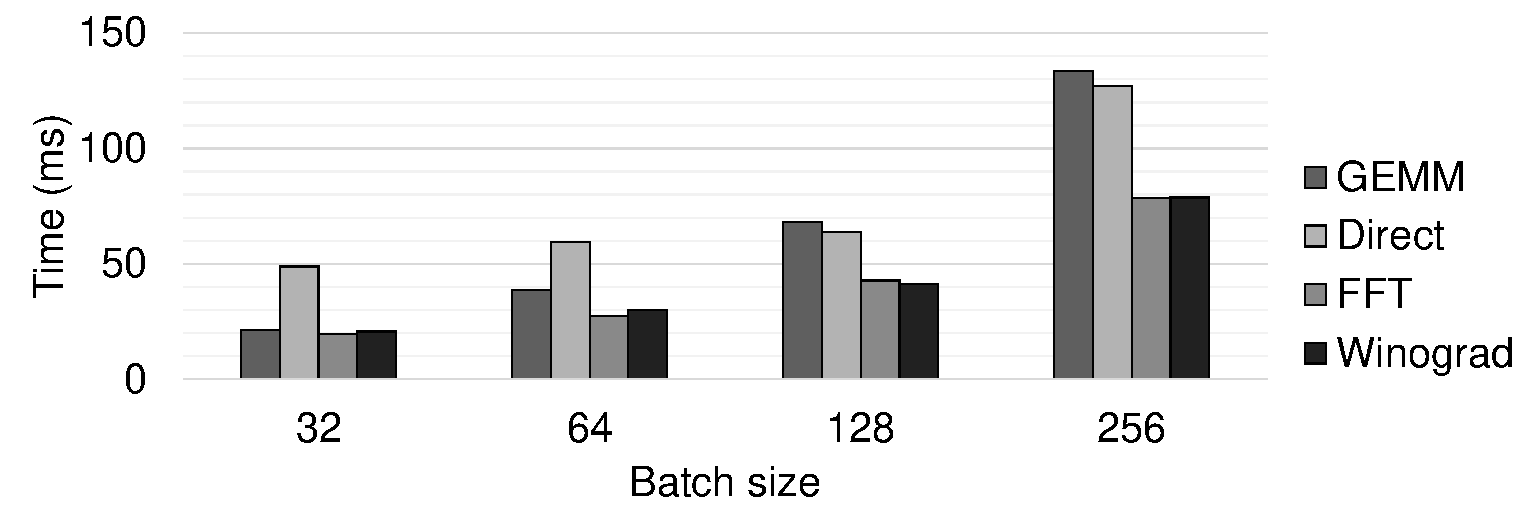
\includegraphics[width=.45\linewidth]{./figures/gpu_time_fwd}
  \label{fig_gpu_time_fwd}}
  \subfloat[The execution time of backward computation] {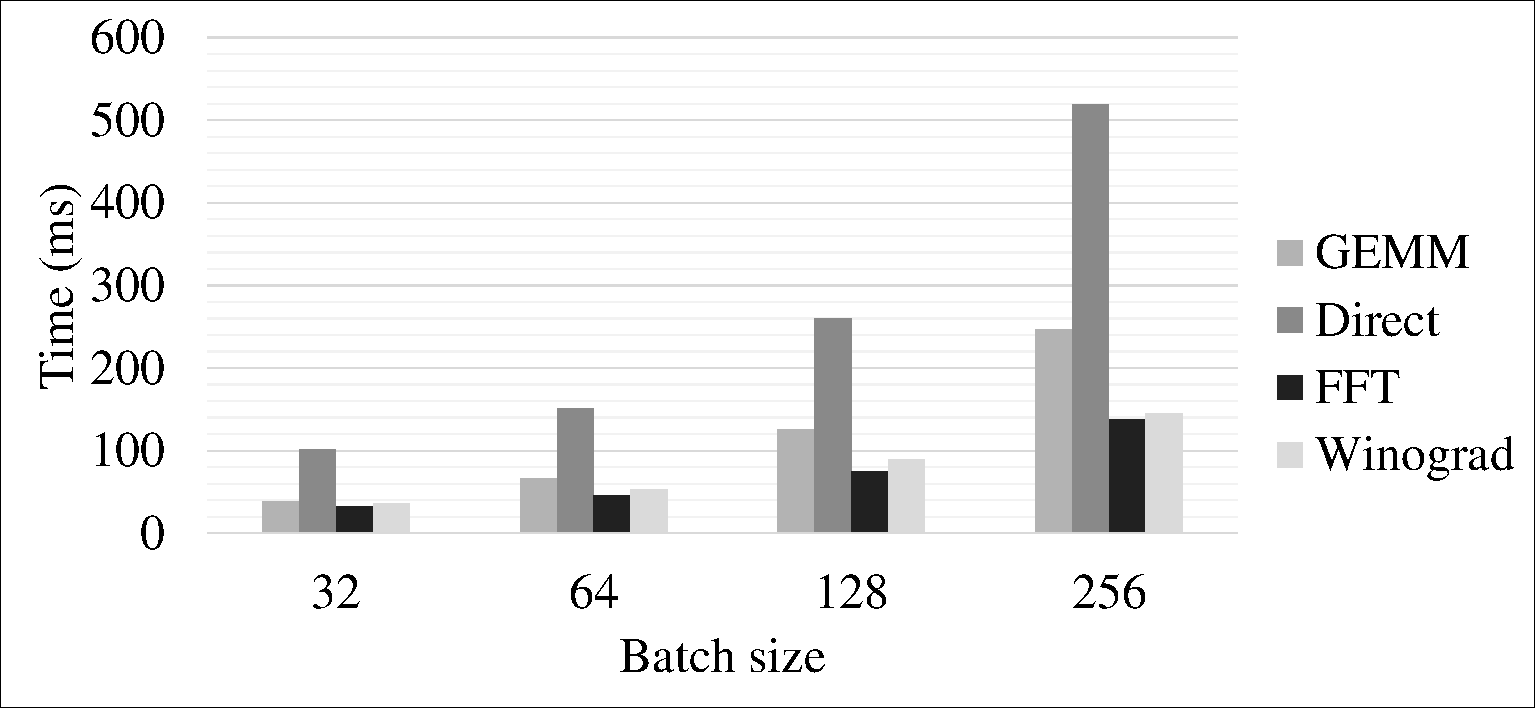
\includegraphics[width=.45\linewidth]{./figures/gpu_time_bwd}
  \label{fig_gpu_time_bwd}}
  \hfil
  \subfloat[The execution time of forward computation from \textsf{conv3} to \textsf{conv5}] {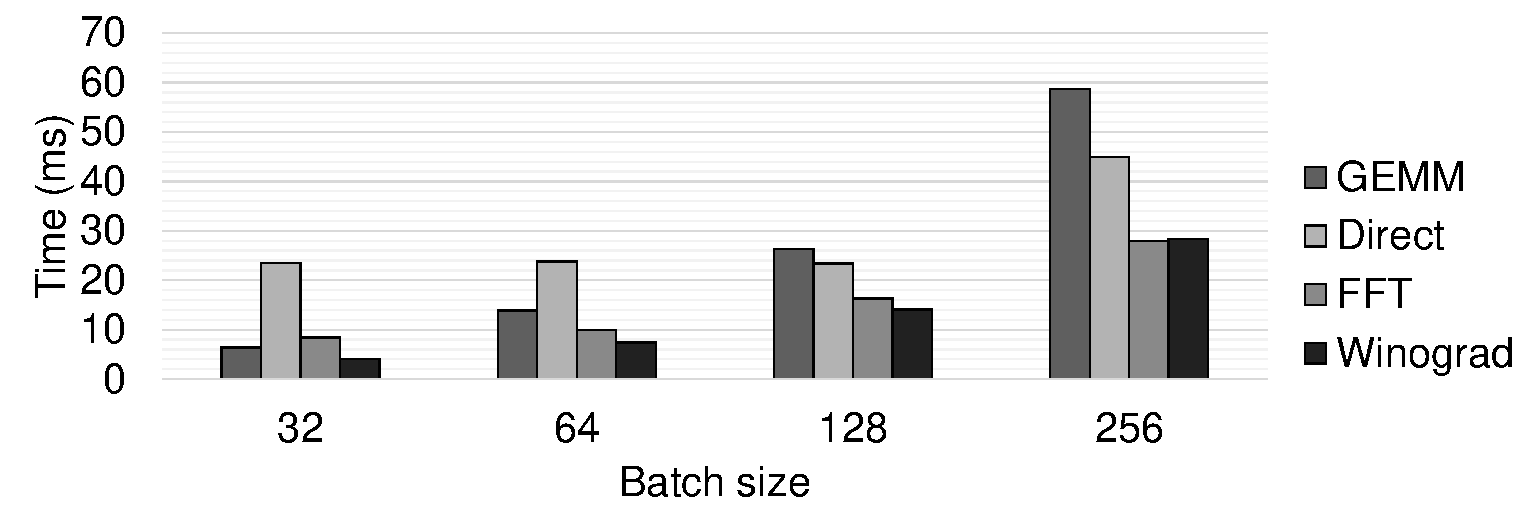
\includegraphics[width=.45\linewidth]{./figures/gpu_time_conv345}
  \label{fig_gpu_time_conv345}}
  \subfloat[Peak GPU memory usage] {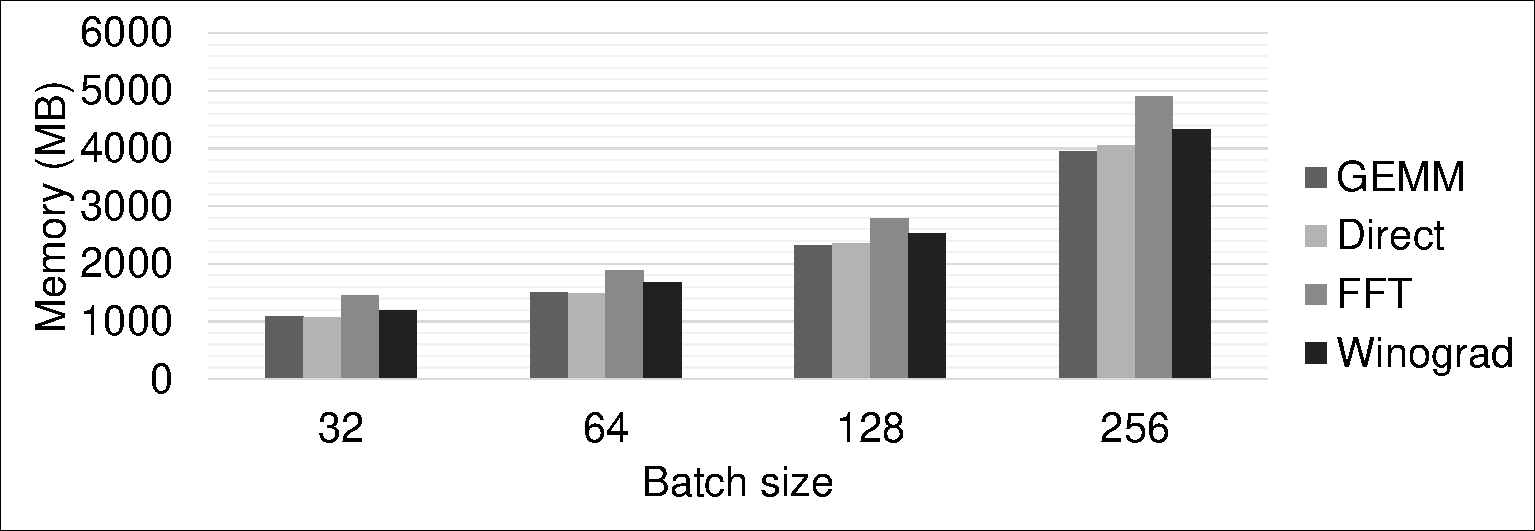
\includegraphics[width=.45\linewidth]{./figures/gpu_mem_kernels}
  \label{fig_gpu_mem}}
  \caption{Execution time and memory usage between different convolution algorithms in training.}
  \label{fig_conv_time}
\end{figure*}%

\section{Effect of Convolution Algorithms}
\label{convolution-algorithms}
In this section, we compare the performance of different convolution algorithms on a single GPU. These algorithms were introduced in Section~\ref{sec:algorithms}. 

\subsection{Backward and Forward convolution}
The backpropagation of a convolution layer requires 2 convolutions: backward data (\textsf{BD}) convolution and backward filter (\textsf{BW}) convolution. Backward data convolution generates gradient input to the previous layer while backward filter convolution computes gradients of the layer parameters. Backward convolution and forward convolution of a convolution layer are symmetric. Hence theoretically the backward computation time should be a double of the forward computation time. Since \textsf{BW} convolution has to write gradients for every parameter of the layer, it is more memory intensive than the others. \Comment{added a subsection for backward convolution}

\subsection{Execution Time}
Figure~\ref{fig_conv_time} shows execution time comparisons between GPU kernels of different convolution algorithms (\textsf{GEMM}, \textsf{Direct}, \textsf{FFT}, and \textsf{Winograd}) on a single GPU. We vary the batch size from 32 to 256. Since the convolution layers take most of the execution time in a CNN, using an efficient convolution algorithm in the CNN model is an important design decision. All comparisons are done with AlexNet built by Torch 7 because currently it is the only framework that officialy supports newest versions of cuDNN and Cuda-convnet3. Randomly generated images are used for the input to remove the I/O latency. The forward and backward computation times are measured and averaged for 100 iterations (\textit{i.e.}, batches). 

\textsf{Winograd} and \textsf{FFT} perform better than \textsf{Direct} or \textsf{GEMM} most of the time as shown in Figure~\ref{fig_conv_time} (a), (b), and (c). Since many recent CNN models use $3 \times 3$ kernel for convolution layers\cite{vgg}, the forward computation time of \textsf{conv3},  \textsf{conv4} and \textsf{conv5} is separately measured in Figure~\ref{fig_gpu_time_conv345}.

The total training time (the forward computation time + the backward computation time) of \textsf{FFT} is the best for all batch sizes. However, for $3 \times 3$ convolution kernels with small batch sizes, \textsf{Winograd} performs better than \textsf{FFT} while \textsf{FFT} scales better with large batch sizes. In addition, \textsf{Direct} (\textit{i.e.}, cuda-convnet) scales bad when the batch size is smaller than 128 while \textsf{GEMM} sclaes almost linearly.

Figure~\ref{fig_gpu_mem} shows peak GPU memory usage for each convolution algorithms. \textsf{FFT} occupies the most GPU memory, using about 20\% more memory than \textsf{GEMM}. 

\begin{figure}[htbp]
  \centering
  \subfloat[The execution time of the forward computation] {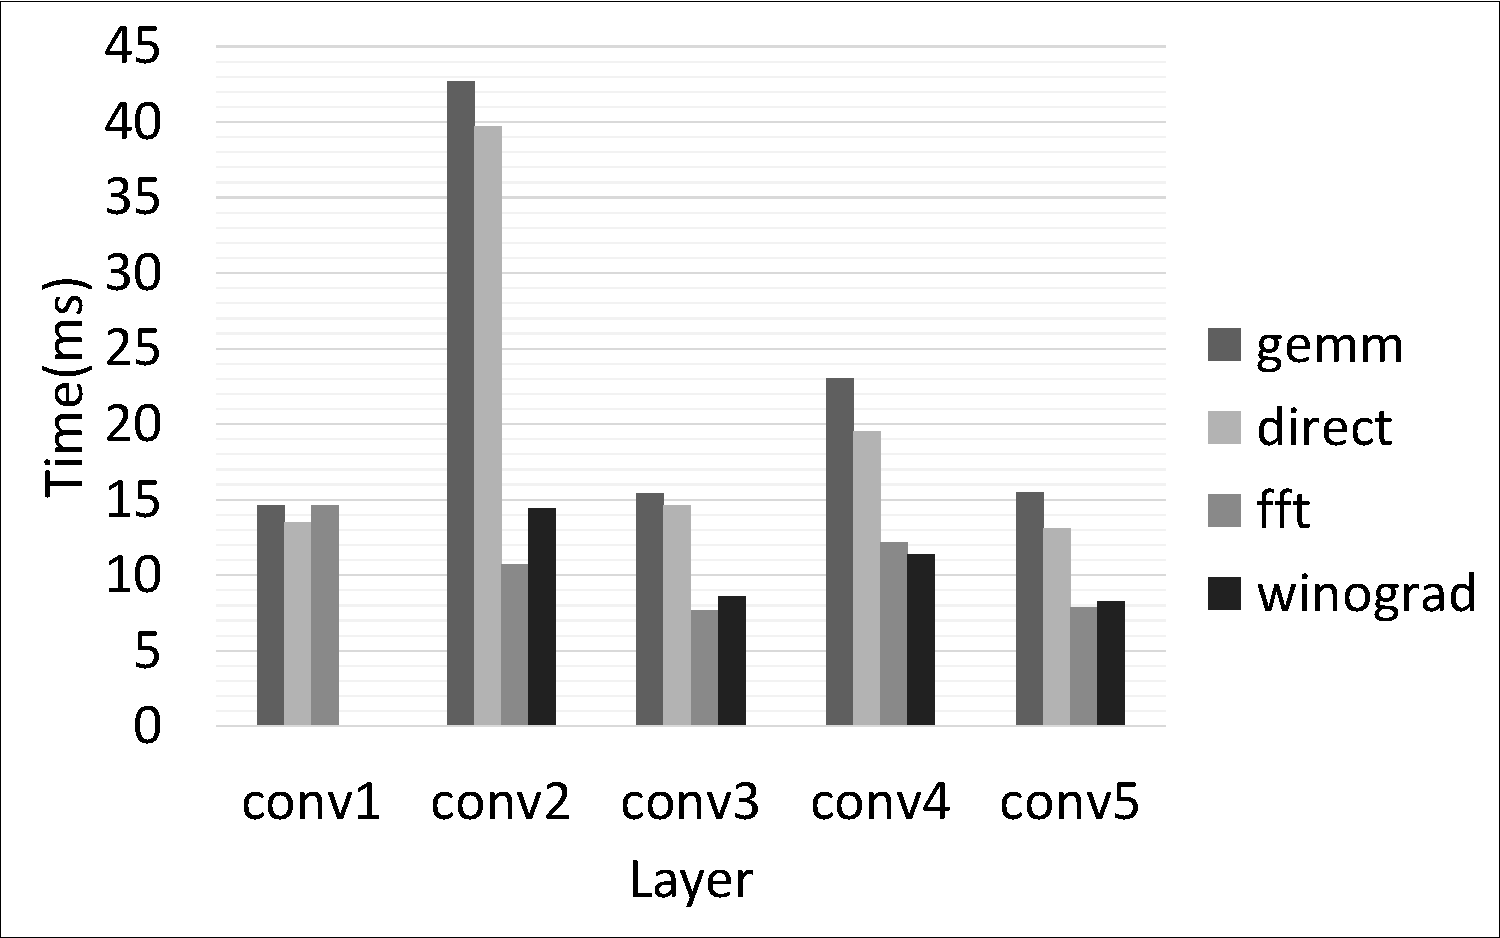
\includegraphics[width=.9\linewidth]{./figures/layerwise_fwd}
  \label{fig_layerwise_fwd}}

  \subfloat[The execution time of the backward computation] {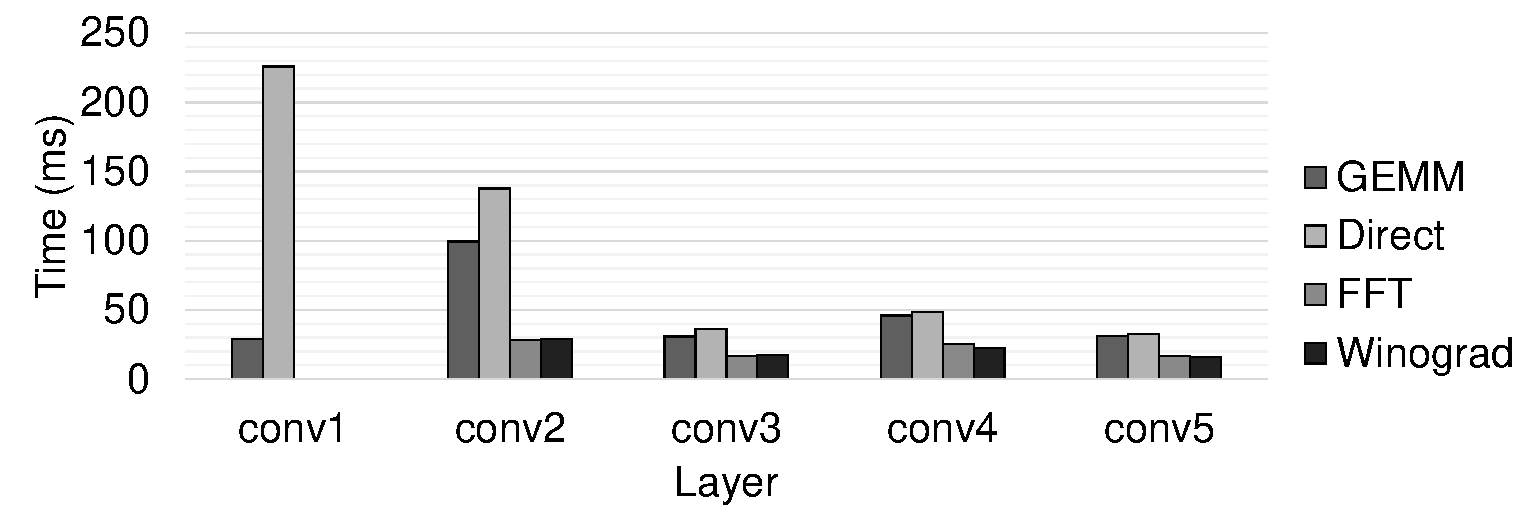
\includegraphics[width=.9\linewidth]{./figures/layerwise_bd}
  \label{fig_layerwise_bd}}

  \subfloat[FP operation count in the forward computation] {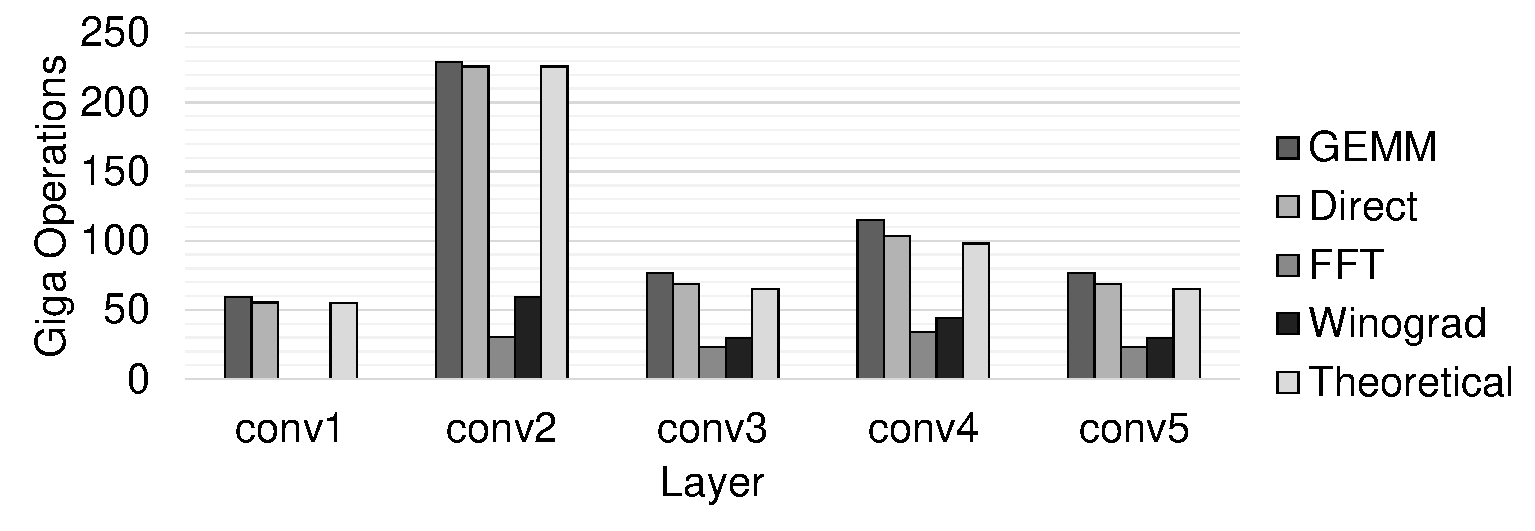
\includegraphics[width=.9\linewidth]{./figures/layerwise_flop_count}
  \label{fig_layerwise_flop_count}}%fixed typo

  \subfloat[Compute-memory ratio of Backward filter convolution kernels] {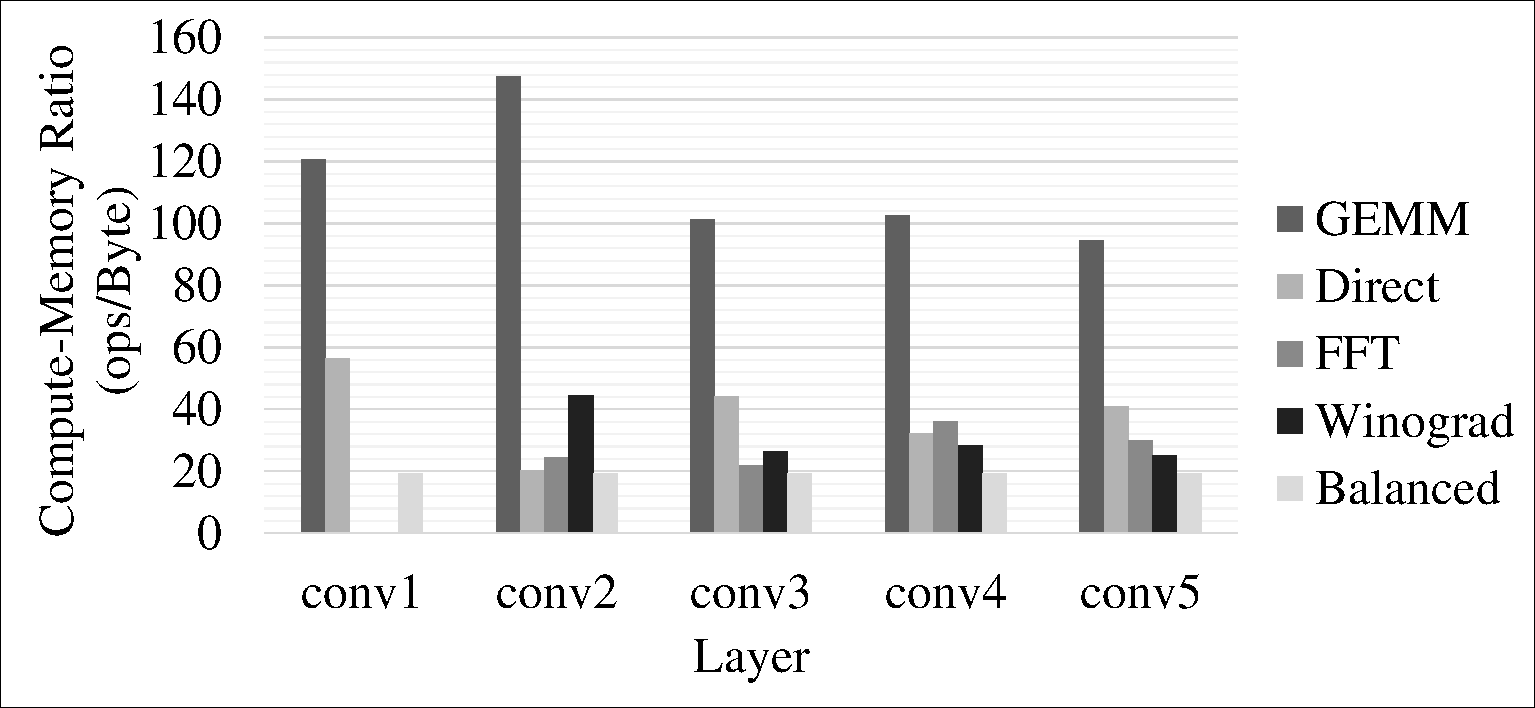
\includegraphics[width=.9\linewidth]{./figures/layerwise_mem_compute}
  \label{fig_layerwise_mem_compute}}%compute-memory ratio chart added

  \caption{Layerwise analysis of different convolution algorithms.}
  \label{fig_layerwise}
\end{figure}

\subsection{Layerwise Analysis}

Figure~\ref{fig_layerwise} shows layerwise analysis of different convolution algorithms on a single GPU. The batch size is set to 256, and the NVIDIA nvprof profiler is used to gather statistics.

As shown in Figure~\ref{fig_layerwise_bd}, the main performance limiter of \textsf{Direct} (\textit{i.e.},cuda-convnet) is the backward computation in \textsf{conv1} layer. The reason of the slowdown is low parallelism in GPU kernels of \textsf{Direct} that implement \textsf{conv1} layer. While NVIDIA Titan X has 3072 CUDA cores, the number of CUDA theads in the GPU kernels is only 1024. This make \textsf{Direct} slower than other algorithms in \textsf{conv1}. 

{\bf Floating-point operation count}. Figure~\ref{fig_layerwise_flop_count} compares floating-point (FP) operation counts of different convolution algorithms in the forward computation. The count is exactly the same in the backward computation kernels. The numbers are measured with the NVIDIA nvprof profiler. \textsf{Theoretical} stands for the theoretically computed count. The result tells us that \textsf{FFT} is usually the fastest because of much less FP operation count (\textit{i.e.}, much less algorithm complexity). Especially, \textsf{FFT} is much faster than others in \textsf{conv2} with $5 \times 5$ convolution filter because the complexity of the FFT algorithm does not depend on the filter size. \textsf{Winograd} also reduces FP operation count by more than half. Thus, its performance is comparable to \textsf{FFT} in the layers with $3 \times 3$ convolution filters (\textsf{conv3}, \textsf{conv4}, and \textsf{conv5}).

{\bf Compute-memory Ratio}. The theoretical maximum FP throughput of NVIDIA Titan X is 6 TFLOPS (floating-point operations per second), and maximum memory bandwidth is 336GB/s. Therefore balanced compute-memory ratio of Titan X is 18.3 FP operations per byte. Fig~\ref{fig_layerwise_mem_compute} shows compute-memory ratio of \textsf{BW} convolution kernels with the balanced ratio of Titan X. We divide FP operation counts to the device memory transaction bytes to calculate compute-memory ratio of the kernels. Since other convolution kernels are less memory intensive than \textsf{BW} convolution, the result indicates that convolution algorithms are compute intensive on a GPU rather than memory intensive. Therefore reduced algorithm complexity of \textsf{FFT} and \textsf{Winograd} result in faster convolutions. \Comment{//changed into compute-memory ratio}

\subsection{Summary}
We conducted layerwise kernel comparison of different convolution algorithms. The convolution kernels have high compute-memory ratio, indicating that they are compute intensive. \textsf{FFT} and \textsf{Winograd} perform significantly better than \textsf{GEMM} or \textsf{Direct} due to reduced algorithm complexity. \textsf{FFT} scales better on large batch and filter sizes while \textsf{Winograd} scales better on smaller batch and filter sizes. Carefully choosing a convolution kernel can make more than $4\times$ difference in a layer computation time. \Comment{//summary for analysis B updated}
\section{Multi-GPU Support}
\label{multi-GPU}
In this section, we characterize the performance of AlexNet built by different deep learning frameworks on multiple GPUs. AlexNet is trained on each framework with one, two, and four GPUs in this experiment. We exploits the data parallelism (explained in Section~\ref{sec:multiGPU-parallelism}) already available in the frameworks. Since Theano does not support mutiple GPUs, we compare only Caffe, CNTK, TensorFlow, and Torch. To train AlexNet, we select the fastest option based on the characteristics on a single GPU in Section~\ref{sec:singlGPU}

To exploit data parallelism, a GPU (say $GPU_0$) gathers intermediate gradient values to update network parameters stored in other GPUs ($GPU_1$, $GPU_2$, and $GPU_3$, assuming four GPUs). If gradients are gathered sequentially going through each GPU, the number of communications for gradient transfer between $GPU_0$ and other GPUs is $O(N-1)$, where $N$ is the number of GPUs. However, if gradients are gathered \Comment{with the parallel reduction algorithm}\cite{harris2007optimizing}, it is $O(\log{N})$ under the assumption that data trasfers can be parallelized if the source and destination GPUs are distinct. As long as a different GPU uses a different set of PCI-E lanes, the PCI-E bus has such property. Thus, our system supports the parallel reduction algorithm.

Ideally, the training time of AlexNet is expected to be reduced to $\frac{1}{N}$ if $N$ GPUs are used. However, this is not true because of the data trasfer caused by the gradient data exchange.
Since the size of gradient data in our AlexNet is about 250MB, the gradient transfer between two GPUs takes about 45ms. This is not negligible considering that one forward and backward computation takes  about 200ms with a batch size of 256.

\begin{figure*}[htbp]
  \centering
  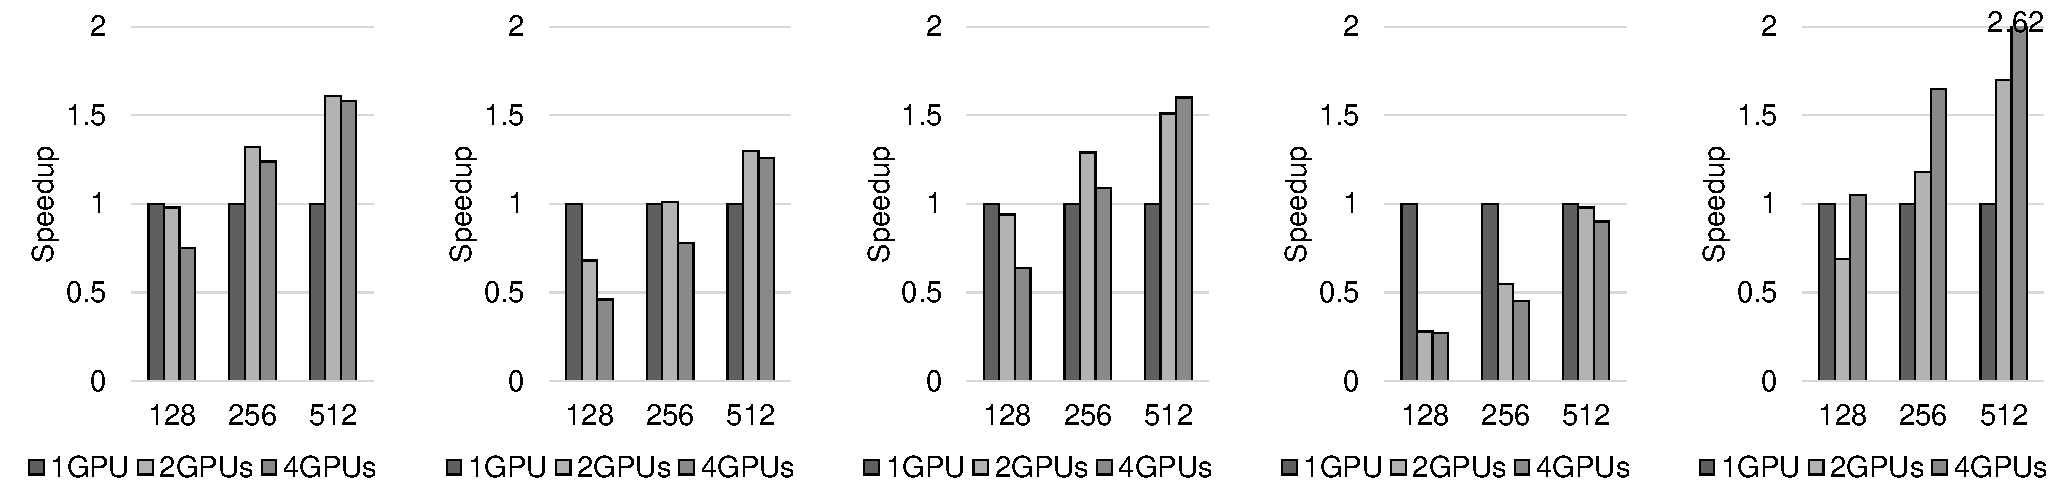
\includegraphics[width=.9\linewidth]{./figures/MG}
\caption{Speedup (over a single GPU) of multi-GPU training of AlexNet built by each framework.}
\label{fig_mg}
\end{figure*}

Figure~\ref{fig_mg} shows speedup obtained by multi-GPU training of our AlexNet built by each framework with different batch sizes and numbers of GPUs. We see that a bigger batch size makes the speedup higher. A batch size of 128 makes Caffe and Torch on two or four GPUs much slower than on a single GPU. A bigger batch size makes the computation time in each GPU longer. However, the number and size of data transfer is fixed because the number of network parameters remains the same. Thus, it is beneficial to use a bigger batch size.

We also see that the scalability of each framework is quite poor. The speedup of using four GPUs is slower than or comparable to that of using two GPUs for all frameworks. \Comment{The reason is, gradient transfer when using four GPUs still takes twice longer than using two GPUs, even though we use the $O(log N)$ algorithm to transfer data between GPUs.}

Torch and TensorFlow have comparable execution time on a single GPU. However, TensorFlow achieves higher speedup than Torch. Since TensorFlow handles gradients of each layer as an individual tensor, the gradients of each layer are transfered as soon as the backward computation of that layer finishes. On the other hand, Torch (and Caffe) references gradients of the entire network as a whole. Thus, it starts data transfer after all backward computations finish. That is, TensorFlow has more data transfer and computation overlapping.

\Comment{CNTK is special in terms of its multi-GPU support. Intermediate gradient values are gathered in the host memory, instead of the parallel reduction algorithm. Although data transfers can be parallelized, gradients are summed up by CPU and it takes much longer than computation time in GPUs. Thus, using any number of GPUs is slower than single GPU training.}

\Comment{Instead of using better reduction, they developed 1bit-SGD\cite{1-bit-stochastic-gradient-descent-and-application-to-data-parallel-distributed-training-of-speech-dnns}. In 1bit-SGD, only one bit per gradient is transfered, reducing memory transfers and CPU computation by a factor of 32 compared to when using the single-precision FP format. This greatly improves scalability to almost linear scale, at the cost of slow convergence.}

\subsection{Summary}

\Comment{We observed that current multi-GPU scalability of frameworks is bad and has many possibilities to be improved. TensorFlow-like data transfer and computation overlapping will be helpful to improve the performance of the framework on a multi-GPU context. Reducing the size of gradients by using approximating the exact value with less accuracy (\textit{e.g.}, using the half-precision FP format or only 1-bit like CNTK) will also improve scalability a lot. Reducing the number of gradients by resizing the CNN model and pruning will also work, especially in fully-connected layers because they contain more than 90\% of network parameters.}

\section{Conclusions}


\section*{Acknowledgment}

This work was supported by the National Research Foundation of Korea (NRF) grant funded by the Ministry of Science, ICT \& Future Planning (MSIP) (No. 2013R1A3A2003664), PF Class Heterogeneous High Performance Computer Development through the NRF funded by the MSIP (NRF-2016M3C4A7952587), and BK21 Plus for Pioneers in Innovative Computing (Dept.\ of Computer Science and Engineering, SNU) through the NRF funded by the Ministry of Education (21A20151113068). ICT at Seoul National University provided research facilities for this study.

\bibliographystyle{IEEEtran}
\bibliography{IEEEabrv,ispass17}
%\nocite{*}

\end{document}
